
\chapter{Martedì 23/03/2021}
\section{Punti su cui stare attenti nella prova pratica} Negli esercizi di traduzione della prova d'esame ci sono due punti ostici:
\begin{enumerate}
	\item uso della MOV/LEA (quando uso una cosa e quando un'altra);
	\item capire più nel dettaglio cosa succede quando una funzione restituisce valori di tipo struttura/classe/unione.
\end{enumerate}
Il primo punto lo abbiamo già affrontato, vediamo il secondo. 
\subsection{Funzioni che restituiscono strutture/classi per valore}
\paragraph{Esempio 1} Supponiamo di voler fare la seguente somma (dove \emph{a} e \emph{b} sono interi)
\[a+b\]
sappiamo che in C++ ogni espressione ha un \emph{tipo} e un \emph{valore}. In questo caso il tipo è \emph{intero} e il valore è il risultato della somma. Questo valore di tipo intero va messo da qualche parte, l'espressione non ci dice cosa ne dobbiamo fare. Se invece indico
\[c=a+b\]
sappiamo che il risultato dovrà essere messo nella variabile \emph{c}. Precisamente:
\begin{enumerate}
	\item memorizzo da qualche parte l'unico risultato intermedio, $a+b$;
	\item copio il risultato intermedio dal luogo in cui l'abbiamo salvato all'indirizzo di \emph{c}.
\end{enumerate}
\paragraph{Esempio 2} Consideriamo la seguente espressione...
\[e=(a+b) \times (c+d)\]
che non può essere calcolata in un colpo solo. Abbiamo tre valori temporanei:
\begin{itemize}
	\item $a+b$
	\item $c+d$
	\item $(a+b) \times (c+d)$
\end{itemize} 
Potremo sbarazzarci di questi valori dopo il loro utilizzo.
\paragraph{Se avessi oggetti?} Supponiamo che \emph{a} e \emph{b} non siano interi, ma istanze di una presunta classe \emph{matrice}. Operator+ è una funzione che ha in ingresso due istanze della classe \emph{matrice} e ne restituisce una terza. 
\[C=A+B\]
Tutti i ragionamenti fatti prima rimangono validi, soprattutto per quanto riguarda i valori intermedi: ho istanze intermedie che devono essere collocate da qualche parte. 
\paragraph{Quali sono le situazioni che possono manifestarsi con questi risultati intermedi?}
\begin{itemize}
	\item Il risultato intermedio ha dimensione inferiore a 16byte: bastano semplicemente i registri.
	\item Il risultato intermedio è più grande di 16byte: dobbiamo creare un vero e proprio \emph{oggetto temporaneo} e allocarlo in memoria. L'oggetto in questione è creato ed eliminato automaticamente dal compilatore, senza esplicita indicazione del programmatore
\end{itemize}
\subsection{Esercizio dalle diapositive di Frosini con struttura superiore a 16byte}
\begingroup
\small
\begin{framed}
	\begin{multicols}{2}
		\noindent \textbf{Codice C++}
		\begin{verbatim}
			// file es12a.cpp
			#include"servi.cpp"
			struct s { int n1; int n2; char a[10];  };
			
			extern "C" s fstruct(int a, char c);
			extern "C" void scriviris(s& ss) { 
				int i;
				scriviint(ss.n1);  scriviint(ss.n2);
				for (i=0; i<10; i++)
				scrivichar(ss.a[i]);
				nuovalinea();
			}
			
			int main() { 
				s sa;
				sa = fstruct(5, 'a');
				scriviris(sa);
				return 0;
				# la struttura non viene letta,
				# ma restituita da fstruct()
			};
			
			// file es12b.cpp
			struct s { int n1; int n2; char a[10]; };
			extern "C" s fstruct(int a, char c) { 
				int i; s st;
				st.n1 = a; st.n2 = 2*a;
				for (i=0; i<10; i++) 
				st.a[i] = c+i;
				
				return st;
			}
		\end{verbatim}
	\end{multicols}
\end{framed}
\textbf{Traduzione della funzione \emph{fstruct}}
\begin{multicols}{2}
	\begin{verbatim}
		.global _Z7fstructic
		_Z7fstructic: 
		push %rbp
		mov %rsp, %rbp
		sub $48, %rsp
		mov %rdi, -8(%rbp)
		mov %esi, -16(%rbp)
		mov %dl, -12(%rbp)
		
		# ...
		
		lea -40(%rbp), %rsi
		mov -8(%rbp), %rdi
		mov $5, %rcx
		rep movsl
		
		mov -8(%rbp), %rax
		leave 
		ret
	\end{verbatim}
\end{multicols}
\begin{itemize}
	\item Scriviamo il nome della funzione
	\begin{verbatim}
		_Z7fstructic
	\end{verbatim}
	\item Dobbiamo restituire un valore più grande di 16byte, quindi siamo costretti a introdurre un nuovo parametro implicito. Questo parametro, come l'altro già visto (\emph{this}), sarà memorizzato nel primo registro disponibile. Seguono i parametri di ingresso e le variabili locali. Vediamo il record di attivazione
	\begin{center}
		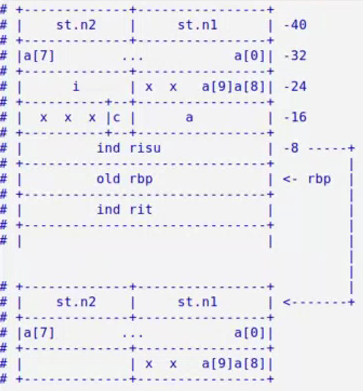
\includegraphics{img/43.PNG}
	\end{center}  
	solito prologo
	\begin{verbatim}
		push %rbp
		mov %rsp, %rbp
		sub $48, %rsp
	\end{verbatim}
	\item Copiamo i parametri
	\begin{verbatim}
		mov %rdi, -8(%rbp) # indirizzo che dicevamo
		mov %esi, -16(%rbp) 
		mov %dl, -12(%rbp)
	\end{verbatim}
	\item Andiamo direttamente alla \emph{return}, questione bollente. Il valore da restituire sono le ultime due righe e mezzo in cima alla pila, più di 16byte. La soluzione migliore è utilizzare le istruzioni per le stringhe viste a Reti logiche (ricordiamoci che fare una cosa con una singola istruzione invece che con più istruzioni è sinonimo di efficienza). 
	\begin{verbatim}
		lea -40(%rbp), %rsi
		mov -8(%rbp), %rdi
		mov $5, %rcx
		rep movsl
	\end{verbatim}
	\begin{itemize}
		\item Poniamo nel registro \emph{rsi} la source (l'indirizzo dell'area di memoria relativa ad \emph{st})
		\item Poniamo nel registro \emph{rdi} la destination (l'indirizzo dell'area di memoria dove porre il valore restituito, in questo caso l'indirizzo è il contenuto di un'area di memoria).
		\item Chiamiamo la \emph{movsl} accompagnandola col prefisso di replicazione \emph{rep}. Quest'ultima decrementa \emph{rcx}, posto uguale a 5, e garantisce l'esecuzione ripetuta della movsl finchè rcx non sarà uguale a zero. La \emph{movsl}, ad ogni iterazione, incrementa l'indirizzo posto in rdi e in rsi.
	\end{itemize}
	\begin{framed}
		\item \textbf{Convenzione}: si restituisce mediante \emph{rax} l'indirizzo di ritorno (quello che abbiamo ricevuto in ingresso)
		\begin{verbatim}
			mov -8(%rbp), %rax
		\end{verbatim}
		L'indirizzo non può essere preso da \emph{rdi}, visto che è stato sporcato dalla \emph{movsl}.
	\end{framed}
	\item Concludiamo allo stesso modo
	\begin{verbatim}
		leave
		ret
	\end{verbatim}
\end{itemize}
\paragraph{Traduzione della funzione \emph{main}} Svestiamo i panni del chiamato e indossiamo quelli del chiamante
\begin{multicols}{2}\begin{verbatim}
		.global main
		main:
		push %rbp
		mov %rsp, %rbp
		sub $48, %rsp
		
		# fstruct(5, `a') <--- temp
		lea -48(%rbp), %rdi
		mov $5, %esi
		mov $'a', %dl
		call _Z7fstructic
		
		# sa = temp
		lea -48(%rbp), %rsi
		lea -24(%rbp), %rdi
		mov $5, %rcx
		rep movsl
		
		# ...
		
		xorl %eax, %eax
		leave
		ret
	\end{verbatim}
\end{multicols}
\begin{center}
	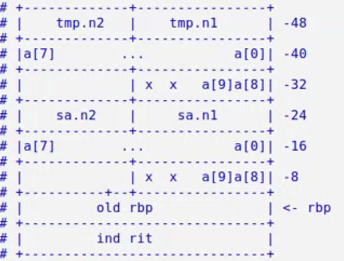
\includegraphics{img/44.PNG}
\end{center}  
\begin{itemize}
	\item Per quanto riguarda il record di attivazione dobbiamo considerare lo spazio non solo per l'istanza \emph{sa} ma anche per l'istanza \emph{temp} di cui abbiamo detto a inizio lezione.
	\item Solito prologo
	\begin{verbatim}
		push %rbp
		mov %rsp, %rbp
		sub $48, %rsp
	\end{verbatim}
	\item Scriviamo l'assegnamento
	\begin{verbatim}
		sa = fstruct(5, `a')
	\end{verbatim}
	La cosa si articola in due parti:
	\begin{itemize}
		\item la creazione dell'istanza \emph{temp}
		\begin{verbatim}
			# fstruct(5, `a') <--- temp
			lea -48(%rbp), %rdi
			mov $5, %esi
			mov $'a', %dl
			call _Z7fstructic
		\end{verbatim}
		chiamo la funzione e ottengo \emph{temp}. Si ricordi che quanto restituito ha dimensione superiore a 16byte, quindi dobbiamo agire in modo diverso rispetto al solito.
		\item l'assegnamento di \emph{sa}
		\begin{verbatim}    
			# sa = temp
			lea -48(%rbp), %rsi
			lea -24(%rbp), %rdi
			mov $5, %rcx
			rep movsl
		\end{verbatim}
		pongo come \emph{sa} il contenuto restituito dalla funzione (cioè \emph{temp}). Gestisco l'assegnamento utilizzando la funzione per stringhe \emph{movsl}, con prefisso di replicazione.
	\end{itemize}
	\item Andiamo direttamente al \emph{return}. Concludiamo allo stesso modo, utilizzando lo \emph{xor} per restituire zero.
	\begin{verbatim}
		xorl %eax, %eax
		leave
		ret
	\end{verbatim}
\end{itemize}
\endgroup

\subsection{Situazioni su cui riflettere}
\subsubsection{Singolo oggetto}
\begin{verbatim}
	C c, x;
	// ...
	x = c
\end{verbatim}
In questo caso non abbiamo bisogno di oggetti temporanei. L'oggetto \emph{c} funge da valore dell'espressione. Non invocheremo il costruttore di copia, se presente, ma l'operatore di assegnamento.
\subsubsection{Chiamata di funzione}
\begin{verbatim}
	C g();
	
	void f() {
		C x;
		// ...
		x = g();
	}
\end{verbatim}
Supponiamo di avere una funzione \emph{g} che restituisce un oggetto di classe \emph{C} per valore. In questo caso è necessario allocare un oggetto temporaneo, per contenere il valore dell'espressione restituita dalla funzione. L'oggetto che andiamo a restituire, come tutti gli oggetti, deve essere 
\begin{itemize}
	\item allocato (svolta dalla funzione \emph{f}, che alloca l'oggetto come se fosse una variabile locale), e
	\item inizializzato (svolta dalla funzione \emph{g},  che restituisce il valore).
\end{itemize}
Abbiamo visto nell'esercizio di Frosini che in caso di oggetti di dimensione superiore a 16byte è necessario introdurre un parametro implicito (come primo parametro, nel registro \emph{rdi}): un puntatore all'oggetto risultato, cioè dove vogliamo porre l'oggetto restituito.
\paragraph{Come traduciamo l'istruzione \emph{return} sicuramente presente in \emph{g}?} 
\begin{enumerate}
	\item Per prima cosa dobbiamo calcolare il valore dell'espressione contenuta nel \emph{return}, ottenendo un altro oggetto di tipo \emph{C}.
	\item La funzione \emph{g} dovrà invocare il costruttore di copia, se presente, sull'oggetto risultato allocato da \emph{f}. Si passa in ingresso il riferimento all'oggetto creato allo step precedente.
	\item Nel caso in cui il costruttore di copia non sia definito la funzione \emph{g} dovrà copiare, membro a membro, \emph{y} nell'oggetto creato da \emph{f} (con le istruzioni per copiare le stringhe viste a Reti logiche).
	\item Si ricordi che la funzione dovrà lasciare l'indirizzo dell'oggetto risultato in \emph{rax}.
\end{enumerate}
Al ritorno da \emph{g} la funzione \emph{f} dovrà completare l'assegnamento tra oggetto risultato e \emph{x}, e poi distruggere l'oggetto risultato. In questo caso va invocato il distruttore, se presente.
\paragraph{Tempo di vita degli oggetti temporanei} Il tempo di vita degli oggetti temporanei \emph{si estende fino al punto e virgola che si trova alla fine dell'istruzione}.
\subsubsection{Costruttore}
Supponiamo di avere un costruttore con parametro \emph{int}, relativo alla classe \emph{C}. Supponiamo di avere \emph{x}, oggetto di tipo \emph{C}
\begin{verbatim}
	x = C(100);
\end{verbatim}
un assegnamento di questo tipo comporta la creazione di un oggetto temporaneo, e l'assegnamento ad \emph{x}. Prendiamo un altro esempio
\begin{verbatim}
	return C(100);
\end{verbatim}
Anche in questo caso viene creato un oggetto temporaneo.  Lo useremo per inizializzare, mediante costruttore di copia, l'oggetto temporaneo allocato dal chiamante della funzione. Il costruttore di copia viene chiamato dalla funzione chiamata relativamente all'oggetto temporaneo allocato dalla funzione chiamante.

\subsubsection{Costruttore di copia}
\paragraph{Cosa succede in presenza di un costruttore di copia?} Negli esercizi dobbiamo stare attenti alla presenza o meno del costruttore di copia. Viene invocato in situazioni dove si inizializza un oggetto di tipo \emph{C} a partire da un altro oggetto dello stesso tipo. Se il costruttore di copia è presente non possiamo fare come visto nell'esercizio di Frosini: dobbiamo demandare la copia al costruttore di copia. Il costruttore di copia va invocato nei seguenti casi...
\begin{enumerate}
	\item \textbf{Assegnamento in caso di dichiarazione dell'oggetto} (costruzione di una nuova istanza a partire da un oggetto già esistente). 
	\begin{verbatim}
		C c = e;
		C c(e);
	\end{verbatim}
	Altri assegnamenti comportano l'uso dell'operatore di assegnamento, non del costruttore di copia.
	\item \textbf{Passaggio di parametri per valore} (cioè poniamo in ingresso, in una funzione, un'istanza della classe)
	\begin{verbatim}
		f(e) <---- parametro di tipo C
	\end{verbatim}
	\item \textbf{Restituzione di valore}. Cosa copiamo? L'espressione che si trova nel return viene copiata nell'oggetto temp. 
	\begin{verbatim}
		return e;
	\end{verbatim}
	Questo significa che nella \emph{fstruct}, in presenza di un costruttore di copia, sarebbe stato necessario chiamarlo, e demandare a lui l'esecuzione della \emph{movsl}. L'allocazione di memoria la fa il chiamante, l'inizializzazione il chiamato, partendo dall'espressione calcolata.
\end{enumerate}

\subsubsection{Elisione dei costruttori di copia (ottimizzazione, RVO ed NRVO)} 
Se rispettiamo queste regole otterremo un gran numero di oggetti temporanei e di invocazioni dei costruttori di copia e dei distruttori. Vediamo il seguente caso:
\begin{verbatim}
	C g() {
		return C(100);
	}
	
	void f() {
		C x = g();
	}
\end{verbatim}
\begin{itemize}
	\item Tra le variabili locali della funzione \emph{f} poniamo \emph{x}, istanza di \emph{C}, e un oggetto temporaneo. Questo mi servirà per valutare l'espressione di \emph{g}
	\item Passo a \emph{g} il solito puntatore implicito (l'indirizzo puntato è quello dell'oggetto temporaneo)
	\item Nella funzione \emph{g} dobbiamo valutare l'espressione nel \emph{return}. Per fare ciò dobbiamo allocare spazio in \emph{g} per un secondo oggetto temporaneo. Su questo oggetto invochiamo il costruttore avente come argomento il parametro intero.
	\item La funzione \emph{g} invoca il costruttore di copia sul primo oggetto temporaneo creato (con riferimento al secondo oggetto) e distrugge il secondo oggetto.
	\item La funzione \emph{f} invoca il costruttore di copia su \emph{x} con riferimento al primo oggetto temporaneo, e infine lo distrugge.
\end{itemize}
\paragraph{Attenzione allo standard} Lo standard prevede che la chiamata dei costruttori di copia possa essere eliminata facendo in modo che si utilizzi, al posto di oggetti temporanei, direttamente le destinazioni. 
\paragraph{Ottimizzazione strana}  L'ottimizzazione dovrebbe rendere il programma più veloce, ma qua si hanno dei \emph{side effects}: pensiamo alle variabili statiche, si ha output diverso in base alla presenza o meno delle ottimizzazioni. Lo standard permette queste ottimizzazioni perché sono troppo importanti: segue che il programmatore deve esserne consapevole.
\begin{framed}\noindent \textbf{Ottimizzazioni svolte}. Lo standard \emph{C++ 17} ha reso obbligatorie tutte le ottimizzazioni che hanno a che fare col costruttore di copia
	\begin{itemize}
		\item \begin{verbatim}
			C c2 = g();
		\end{verbatim}
		non copio in \emph{c2} un oggetto temporaneo, ma costruisco direttamente \emph{c2}.
		\item \emph{Return Value Optimization} (RVO):
		\begin{verbatim}
			return C(100);
		\end{verbatim}
		non creo un oggetto temporaneo.
	\end{itemize}
	Ulteriore ottimizzazione, non obbligatoria, è la \emph{Named Return Value Optimization} (NRVO):
	\begin{verbatim}
		C g() {
			C c(100);
			c.do_something();
			return c;
		}
	\end{verbatim}
	questo tipo di ottimizzazione è sofisticata (contrariamente alla RVO non guardo solo il return, ma tutta la funzione). Non alloco \emph{c}, ma utilizzo direttamente l'oggetto temporaneo allocato dal chiamante (indicato in ingresso come parametro implicito, in rdi). 
\end{framed}
\clearpage 

\noindent \textbf{Traduzione della \emph{fstruct} con la \emph{Named Return Value Optimization}}
\begin{multicols}{2}
	\begin{verbatim}
		.global _Z7fstructic
		_Z7fstructic:
		push %rbp
		mov %rsp, %rbp
		sub $32, %rsp
		mov %rdi, -8(%rbp)
		mov %esi, -16(%rbp)
		mov %dl, -12(%rbp)
		
		# mov st.n1 = a ottimizzato
		mov %esi, (%rdi)
		# mov st.n 2= 2*a 
		mov %esi, %eax
		sal $1, %eax
		mov %eax, 4(%rdi)
		
		# for ...
		
		# return st
		mov -8(%rsp), %rax
		leave
		ret
	\end{verbatim}
\end{multicols}
\small
\begin{itemize}
	\item Il record di attivazione è di dimensione minore, non si alloca spazio per la variabile temporanea \begin{center}
		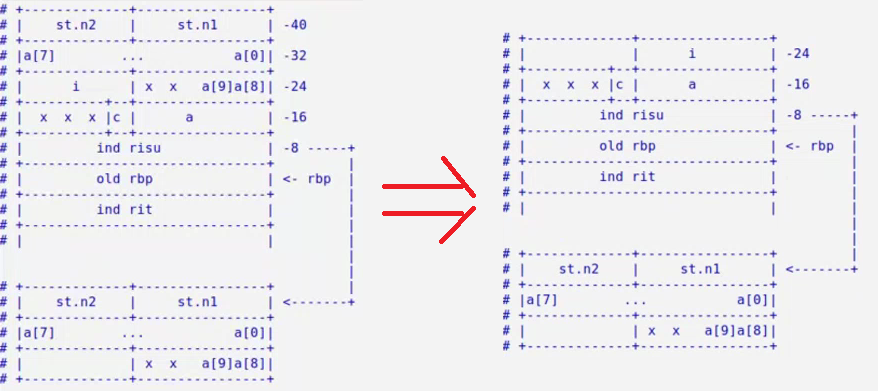
\includegraphics[scale=0.86]{img/45.PNG}
	\end{center}  
	\item Copiamo i parametri
	\begin{verbatim}
		mov %rdi, -8(%rbp) # indirizzo che dicevamo
		mov %esi, -16(%rbp) 
		mov %dl, -12(%rbp)
	\end{verbatim}
	\item Al posto di allocare \emph{st} utilizziamo direttamente l'oggetto in cui poi \emph{st} andrà copiato. 
	\begin{verbatim}
		# mov st.n1 = a ottimizzato
		mov %esi, (%rdi)
		# mov st.n2 = 2*a 
		mov %esi, %eax
		sal $1, %eax
		mov %eax, 4(%rdi)
	\end{verbatim}
	\item Concludiamo restituendo, secondo convenzione, l'indirizzo dell'oggetto allocato dal chiamante
	\begin{verbatim}
		mov -8(%rsp), %rax
		leave
		ret
	\end{verbatim}
\end{itemize}
\normalsize 